\begin{center}
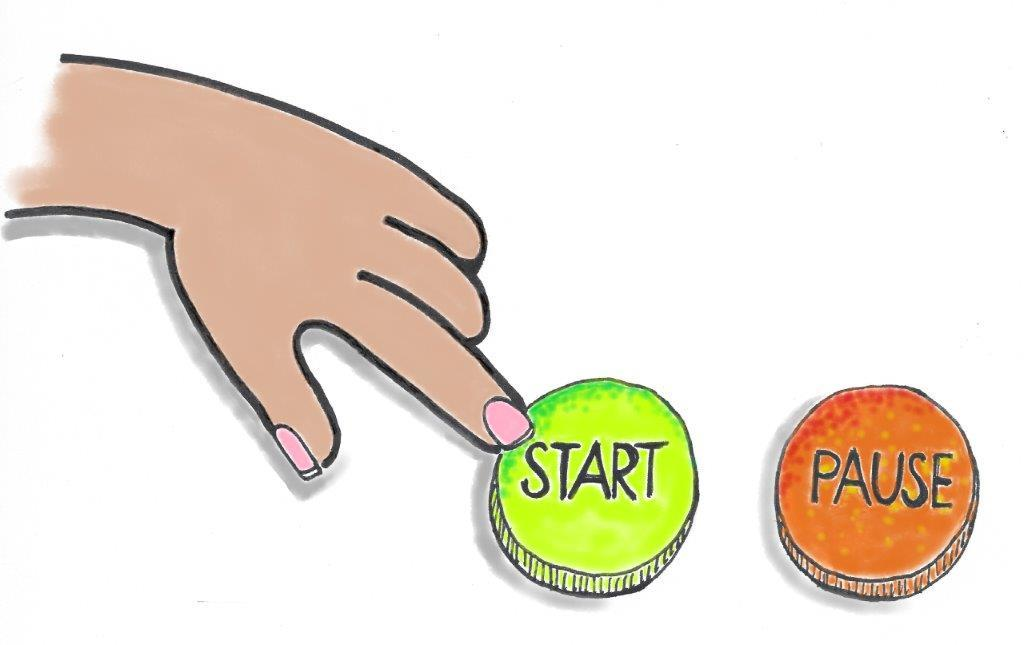
\includegraphics[width=0.4\textwidth]{content/3/chapter7/images/7.png}\\
Cippi开启工作流
\end{center}

在使用co\_return的章节中创建future之前,我们应该理解其控制流。注释使控制流透明。此外,我还提供了在线编译器上提供的程序的链接。

\begin{lstlisting}[style=styleCXX]
// eagerFutureWithComments.cpp

#include <coroutine>
#include <iostream>
#include <memory>

template<typename T>
struct MyFuture {
std::shared_ptr<T> value;
	MyFuture(std::shared_ptr<T> p): value(p) {
		std::cout << " MyFuture::MyFuture" << '\n';
	}
	~MyFuture() {
		std::cout << " MyFuture::~MyFuture" << '\n';
	}
	T get() {
		std::cout << " MyFuture::get" << '\n';
		return *value;
	}

	struct promise_type {
		std::shared_ptr<T> ptr = std::make_shared<T>();
		promise_type() {
			std::cout << " promise_type::promise_type" << '\n';
		}
		~promise_type() {
			std::cout << " promise_type::~promise_type" << '\n';
		}
		MyFuture<T> get_return_object() {
			std::cout << " promise_type::get_return_object" << '\n';
			return ptr;
		}
		void return_value(T v) {
		std::cout << " promise_type::return_value" << '\n';
		*ptr = v;
		}
		std::suspend_never initial_suspend() {
			std::cout << " promise_type::initial_suspend" << '\n';
			return {};
		}
		std::suspend_never final_suspend() noexcept {
			std::cout << " promise_type::final_suspend" << '\n';
			return {};
		}
		void unhandled_exception() {
			std::exit(1);
		}
	};
};

MyFuture<int> createFuture() {
	std::cout << "createFuture" << '\n';
	co_return 2021;
}

int main() {

	std::cout << '\n';
	
	auto fut = createFuture();
	auto res = fut.get();
	std::cout << "res: " << res << '\n';
	
	std::cout << '\n';
}
\end{lstlisting}

调用createFuture(第60行)创建MyFuture实例。MyFuture的构造函数调用(第10行)完成之前,promise promise\_type就会创建、执行和销毁(第21-49行)。promise在其控制流的每一步中都使用可等待的std::suspend\_never(第37和41行),因此从不暂停。为了为后面的fut.get()保存promise的结果(第60行),所以必须对它进行内存分配。此外,使用的std::shared\_ptr的(第9行和第22行)程序不会出现内存泄漏。作为局部变量,fut在第65行超出了范围,C++运行时届时会调用其析构函数。

您可以在\href{https://godbolt.org/z/Y9naEx}{Compiler Explorer}上尝试编译运行该程序。

\begin{center}
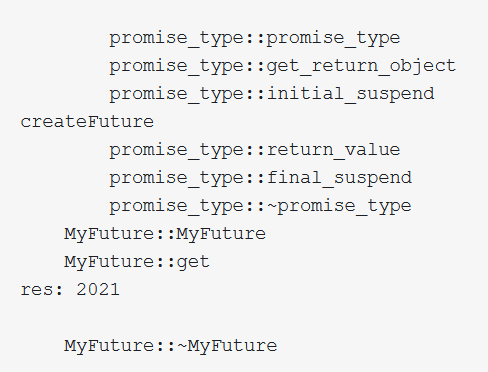
\includegraphics[width=0.4\textwidth]{content/3/chapter7/images/8.png}\\
\end{center}

所呈现的协程立即运行。此外,协程会在调用者的线程中运行。

现在,来让协程变懒惰。

\subsubsubsection{7.2.1\hspace{0.2cm}惰性future}

惰性future是指仅在请求值时才运行的future,来看看需要对eagerFutureWithComments.cpp中的立即协程中进行哪些修改,才能使其变得懒惰。

\begin{lstlisting}[style=styleCXX]
// lazyFuture.cpp

#include <coroutine>
#include <iostream>
#include <memory>

template<typename T>
struct MyFuture {
	struct promise_type;
	using handle_type = std::coroutine_handle<promise_type>;
	
	handle_type coro;
	
	MyFuture(handle_type h): coro(h) {
		std::cout << " MyFuture::MyFuture" << '\n';
	}
	~MyFuture() {
		std::cout << " MyFuture::~MyFuture" << '\n';
		if ( coro ) coro.destroy();
	}
	
	T get() {
		std::cout << " MyFuture::get" << '\n';
		coro.resume();
		return coro.promise().result;
	}

	struct promise_type {
		T result;
		promise_type() {
			std::cout << " promise_type::promise_type" << '\n';
		}
		~promise_type() {
			std::cout << " promise_type::~promise_type" << '\n';
		}
		auto get_return_object() {
			std::cout << " promise_type::get_return_object" << '\n';
			return MyFuture{handle_type::from_promise(*this)};
		}
		void return_value(T v) {
			std::cout << " promise_type::return_value" << '\n';
			result = v;
		}
		std::suspend_always initial_suspend() {
			std::cout << " promise_type::initial_suspend" << '\n';
			return {};
		}
		std::suspend_always final_suspend() noexcept {
			std::cout << " promise_type::final_suspend" << '\n';
			return {};
		}
		void unhandled_exception() {
			std::exit(1);
		}
	};
};

MyFuture<int> createFuture() {
	std::cout << "createFuture" << '\n';
	co_return 2021;
}

int main() {

	std::cout << '\n';
	
	auto fut = createFuture();
	auto res = fut.get();
	std::cout << "res: " << res << '\n';
	
	std::cout << '\n';

}
\end{lstlisting}

我们先来研究一下promise。promise总是在开头(第44行)和结尾(第48行)处挂起。此外,成员函数get\_return\_object(第36行)会创建返回对象,返回给协程createFuture的调用者(第58行)。future MyFuture更有趣,它有一个用来处理promise的句柄coro(第12行)。MyFuture使用这个句柄来管理promise。可以恢复promise(第24行)执行,向promise请求结果(第25行),最后销毁它(第19行)。恢复协程是必要的,因为它不会自动运行(第44行)。当调用端使用fut.get()(第68行)来请求future的结果时,就会隐式地恢复promise(第24行)的运行。

可以在\href{https://godbolt.org/z/EejWcj}{Compiler Explorer}上尝试编译运行该程序。

\begin{center}
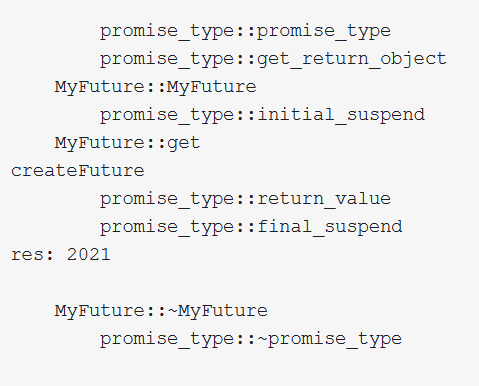
\includegraphics[width=0.4\textwidth]{content/3/chapter7/images/9.png}\\
\end{center}

若调用端对future的结果不感兴趣怎么办?让我们模拟一下。

\begin{lstlisting}[style=styleCXX]
int main() {
	
	std::cout << '\n';
	
	auto fut = createFuture();
	// auto res = fut.get();
	// std::cout << "res: " << res << '\n';
	
	std::cout << '\n';
}
\end{lstlisting}

正如读者们可能猜到的那样,promise永远不会运行,成员函数return\_value和final\_suspend也不会执行。

\begin{center}
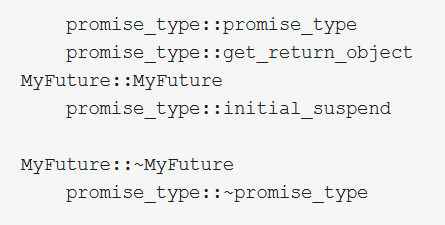
\includegraphics[width=0.4\textwidth]{content/3/chapter7/images/10.png}\\
\end{center}

\begin{tcolorbox}[breakable,enhanced jigsaw,colback=red!5!white,colframe=red!75!black,title={关于数据}]
处理协程的挑战之一是处理协程的生命周期。在前面的eagerFutureWithComments.cpp中,我将协程结果存储在std::shared\_ptr中。这很重要,因为协程会立即执行。

lazyFuture.cpp中,使用final\_suspend总是挂起(第48行):std::suspend\_always final\_suspend()。因此,promise比调用端的生命周期更长,不再需要std::shared\_ptr。所以,从函数final\_suspend返回std::suspend\_never将导致未定义行为。因此,结果的生命周期在调用端请求它之前就结束了。
\end{tcolorbox}

让我们进一步修改协程,并在单独的线程中运行promise。

\subsubsubsection{7.2.2\hspace{0.2cm}在另一个线程上执行协程}

进入协程createFuture之前,因为成员函数initial\_suspend返回std::suspend\_always(第51行),所以协程处于挂起(第66行)状态。因此,promise可以在另一个线程上执行。

\begin{lstlisting}[style=styleCXX]
// lazyFutureOnOtherThread.cpp

#include <coroutine>
#include <iostream>
#include <memory>
#include <thread>

template<typename T>
struct MyFuture {
	struct promise_type;
	using handle_type = std::coroutine_handle<promise_type>;
	handle_type coro;

	MyFuture(handle_type h): coro(h) {}
	~MyFuture() {
		if ( coro ) coro.destroy();
	}

	T get() {
		std::cout << " MyFuture::get: "
	              << "std::this_thread::get_id(): "
	              << std::this_thread::get_id() << '\n';
		std::thread t([this] { coro.resume(); });
		t.join();
		return coro.promise().result;
	}

	struct promise_type {
		promise_type(){
			std::cout << " promise_type::promise_type: "
			          << "std::this_thread::get_id(): "
			          << std::this_thread::get_id() << '\n';
		}
		~promise_type(){
			std::cout << " promise_type::~promise_type: "
			          << "std::this_thread::get_id(): "
			          << std::this_thread::get_id() << '\n';
		}
		
		T result;
		auto get_return_object() {
			return MyFuture{handle_type::from_promise(*this)};
		}
		void return_value(T v) {
			std::cout << " promise_type::return_value: "
			          << "std::this_thread::get_id(): "
			          << std::this_thread::get_id() << '\n';
			std::cout << v << std::endl;
			result = v;
		}
		std::suspend_always initial_suspend() {
			return {};
		}
		std::suspend_always final_suspend() noexcept {
			std::cout << " promise_type::final_suspend: "
			          << "std::this_thread::get_id(): "
			          << std::this_thread::get_id() << '\n';
		return {};
		}
		void unhandled_exception() {
			std::exit(1);
		}
	};
};

MyFuture<int> createFuture() {
	co_return 2021;
}

int main() {

	std::cout << '\n';
	
	std::cout << "main: "
	<< "std::this_thread::get_id(): "
	<< std::this_thread::get_id() << '\n';
	
	auto fut = createFuture();
	auto res = fut.get();
	std::cout << "res: " << res << '\n';
	
	std::cout << '\n';

}
\end{lstlisting}

我在代码中添加了一些注释,显示正在运行的线程的id。lazyFutureOnOtherThread.cpp与前面的程序lazyFuture.cpp非常相似。主要区别在于成员函数get(第19行)。使用std::thread t([this] \{coro.resume();\});(第23行),将在另一个线程上恢复协程的执行。

你可以在\href{https://wandbox.org/permlink/jFVVj80Gxu6bnNkc}{Wandbox}在线编译器上尝试这个程序。

\begin{center}
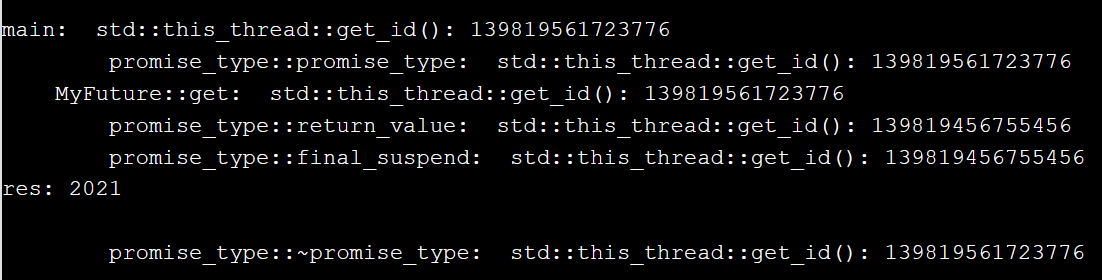
\includegraphics[width=0.8\textwidth]{content/3/chapter7/images/11.png}\\
\end{center}

我想补充一些关于成员函数get的内容。在另一个线程中恢复的promise,必须在返回coro.promise().result之前完成,这一点至关重要。

\hspace*{\fill} \\ %插入空行
\noindent
\textbf{成员函数获取std::thread}
\begin{lstlisting}[style=styleCXX]
T get() {
	std::thread t([this] { coro.resume(); });
	t.join();
	return coro.promise().result;
}
\end{lstlisting}

函数在调用return coro.promise()后将线程t汇入,程序将具有未定义行为。下面函数get的实现中,我使用了std::jthread。std::jthread在超出作用域时可以自动汇入,但这太迟了。

\hspace*{\fill} \\ %插入空行
\noindent
\textbf{成员函数获取std::jthread}
\begin{lstlisting}[style=styleCXX]
T get() {
	std::jthread t([this] { coro.resume(); });
	return coro.promise().result;
}
\end{lstlisting}

这种情况下,调用端很可能在promise使用成员函数return\_value准备promise之前,就得到了结果。result有一个任意值,res也一样。

\begin{center}
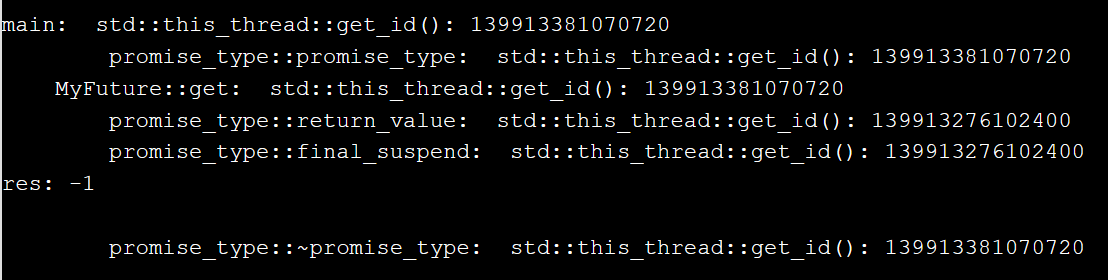
\includegraphics[width=0.8\textwidth]{content/3/chapter7/images/12.png}\\
\end{center}

还有其他方法可以确保线程在返回调用之前完成。

\begin{itemize}
\item 
在其作用域中创建std::jthread。

\begin{lstlisting}[style=styleCXX]
T get() {
	{
		std::jthread t([this] { coro.resume(); });
	}
	return coro.promise().result;
}
\end{lstlisting}

\item 
将std::jthread设置为临时对象

\begin{lstlisting}[style=styleCXX]
T get() {
	std::jthread([this] { coro.resume(); });
	return coro.promise().result;
}
\end{lstlisting}

\end{itemize}

特别说明,我不喜欢最后一个解决方案,因为它可能需要几秒钟,才能意识到刚刚调用了std::jthread的构造函数。

\newpage
